%----------------------------------------------------------------------------
\chapter{The used cyberphysical system}
%----------------------------------------------------------------------------
\section{Usage of the designed software}

The designed monitoring software is made to be part of the system created for the Future Internet Research, Services and Technology project started by ETIK organization. The system is a prototype of a sensor network where the output of sensors can be used to create so called virtual sensors and store the data in a central data store. The system can reason using the ontology built on the sensors. A detailed introduction can be found in this chapter.

\section{Goal of the project}

The project's goal is to show a prototype of a cyberphisical system. It should contain sample sensors, a central database and also a planner, which plans the deployment of the designed new processes or virtual sensors. The system should prove using small example use cases that such a system is feasible to build. The prototype should not need to scale for large amount of sensors.

\section{System architecture}

The system was designed in the following way: 
There are computing or sensing resources called nodes which can provide computational capacity for the new application or sensor output using its sensors. The measurements are sent to the central SOS server and the available free resource information to the RDF store.
The SOS server stores the measurements and provide the data to the other nodes. There is a translation module, which can create the RDF representation of the sensor database for the ontology. 
The RDF store contains the overall architecture of the deployed applications and resource nodes. It also stores the load of each node. 
There is a sensor browser module which users can use to search in the ontology. It is connected to a measurement browser which will display the observations of the selected sensors. 
Users can deploy new application through the planner system. A package shall be uploaded and the planner should automatically deploy it to the chosen node. 
The status of the system can be seen on the implemented monitoring system.

\begin{figure}[h]
	\centering
	%custom
	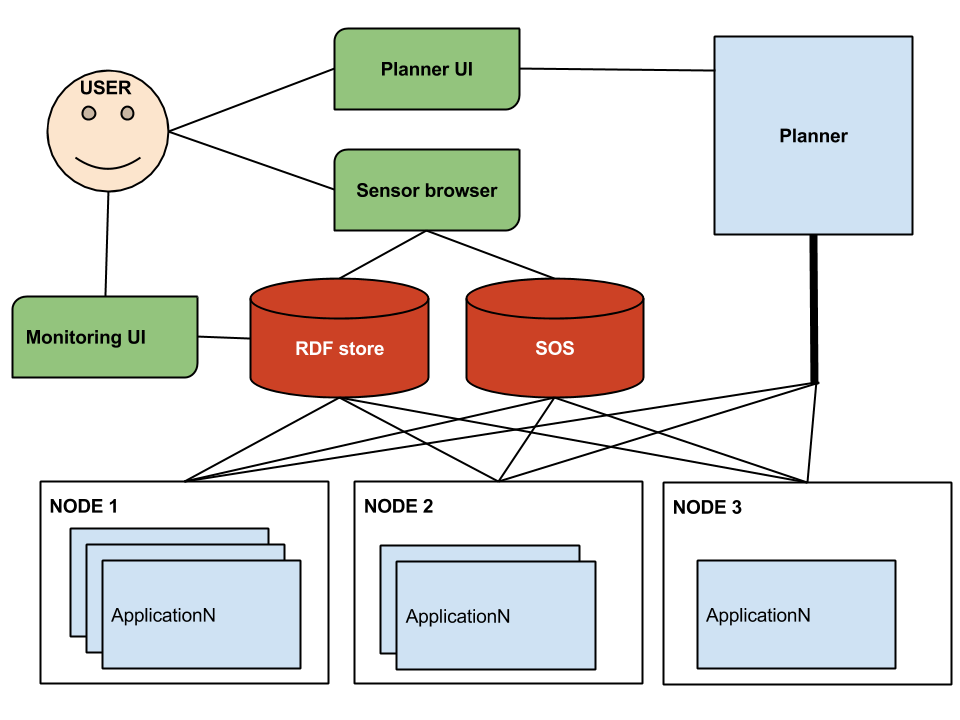
\includegraphics[width=0.9\textwidth]{figures/sysarch.png}
	\caption{System overview\label{fig:sysover}}
\end{figure}

\section{Sensor devices}
The system is using different devices with different capabilities. There are simple microcontrollers and high performance mobile phones integrated in the system. 

The most simple solution is the Arduino Uno board with Ethernet controller. The card has an AVR based microcontroller working inside. It is good for simple measurement. It contains 14 general purpose inputs and outputs from which 6 can be PWM output. It's computing speed is 16Mhz.

The next in computational power is the Raspberry PI computer. This computer was designed to be cheap, reliable and compact, so poor people in developing countries can afford it. There are two models, both of them are fully working desktop computer with 700Mhz ARM cpu. It has:
\begin{itemize}
	\item 3 USB port
	\item 1 CSI port for raw camera input
	\item 1 Composite video output
	\item 1 HDMI output
	\item 1 SD/MMC/SDIO card reader
	\item 8 GPIO port (for UART, SPI, I2C, I2S audio)
\end{itemize} 
 It can run multiple operating systems, like Arch Linux, Raspbian OS, Debian, Slackware, etc. The more expensive model which costs around 35 dollars has a built in Ethernet port.  

The most expensive embedded computer is the BeagleBone in the project. This computer was developed by Texas instruments. It has a 600Mhz ARM Cortex 8 processor with 128 MB of RAM. It has built in features for sound and video processing. It costs around 150 USD. 


\section{Sensor Observation Service}

The sensors communicate with the 52n SOS server using POX GET requests. To reach the service the sensors have to be in the same network or VPN to make the connection secure. The service has its own client installed next to it.

\section{RDF store\label{sec:rdfstore}}

The ontology is stored in an RDF database. It is based on the ontology introduced in the previous Chapter. The SSN Ontology has been extended for the custom use cases. The introduced ontology is called SISRO. It extends the original ontology in two ways:
\begin{itemize}
	\item It describes concepts and relations present in SensorML (and missing from SSN)
	\item It contains hardware details of the sensor devices
\end{itemize}


For easy communication with the sensors and the SOS server, the system can be reached using a custom service.
This Sensor Instance Semantic Registry Service contains the following interfaces:
\begin{itemize}
	\item Collection of Sensor Metadata. This interface contains the metadata for discovering sensors.
	\item System Discovery Interface. This interface is responsible for discovering sensors, searching in them using semantic connections.
	\item Sensor Status Interface. This interface manages the status information of the sensors. This interface makes it possible to search based on Status Information and change states.
	\item Sensor and hardware interconnection interface. Sensors does not have hardware description in SensorML. This interface supports application installation information and reconfiguration.
	\item SPARQL interface. This interface lets users to interact with the database on a low level.	  
\end{itemize}
The layer architecture can be seen on Figure \ref{fig:sisrserv}.	

\begin{figure}[h]
	\centering
	%custom
	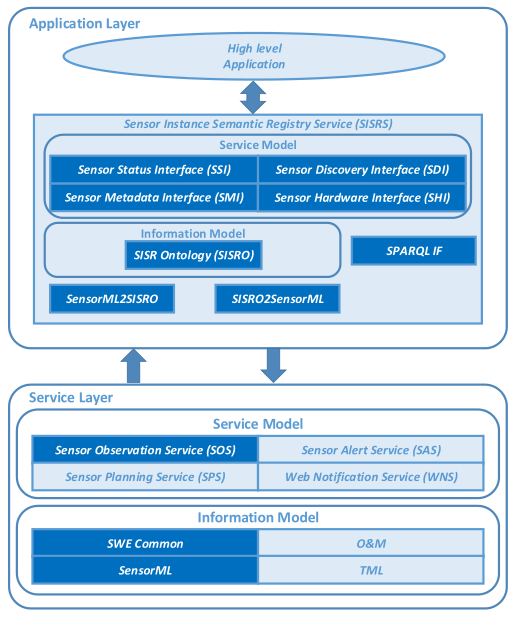
\includegraphics[width=0.7\textwidth]{figures/sisrserv.png}
	\caption{SISR service layers\label{fig:sisrserv}}
\end{figure}
The custom API has the following functions:
\begin{itemize}
\item GetCapabilities(): This function returns the sensor metadata from the database.
\item SearchSensor(): This function makes it possible to query the sensors based on temporal, spatial or topical properties.
\item DescribeSensor(): This function returns the SISRO ontology of a chosen sensor.
\item UpdateSensorInfo(): This function enables modification of sensor metadata.
\item GetSensorStatus(): This function retrieves sensor statuses.
\item SetSensorStatus(): This function lets the users modify sensor statuses.
\item AssignSensor(): This function assigns a sensor to a specific device.
\item RemoveSensor(): This function removes a sensor from the device.
\end{itemize}

However, these services does not contain the necessary features to build the semantic connection between the sensors and their categories. That is why the implemented software uses the RDF databese directly.

\section{Planner}
The planer is a separate module that is capable of deploying different applications to the different resources. It is not used in the monitoring only its results, the deployed application.

\section{Image processing example application}

In the following example a a real life use case of the built cyberphisical system is solved. This example has been implemented in the project itself\cite{g6d1}. 

The goal was to check visual signals in a server room. There was a switch in the room what had blinking LED lights for indicating network connection. In this scenario we would like to monitor these connections only by using the LED indicators. The application is capturing a live video stream from the server room. In the video stream, the LEDs are seen. The user can specify the position of the monitored LEDs. The observations are categorized into 3 different categories:
\begin{itemize}
	\item Switched off - The LED hasn't been turned on since 5 seconds
	\item Blinking
	\item Turned on - The LED hasn't been turned off in the past 5 second
\end{itemize}

\begin{figure}[h]
	\centering
	%custom
	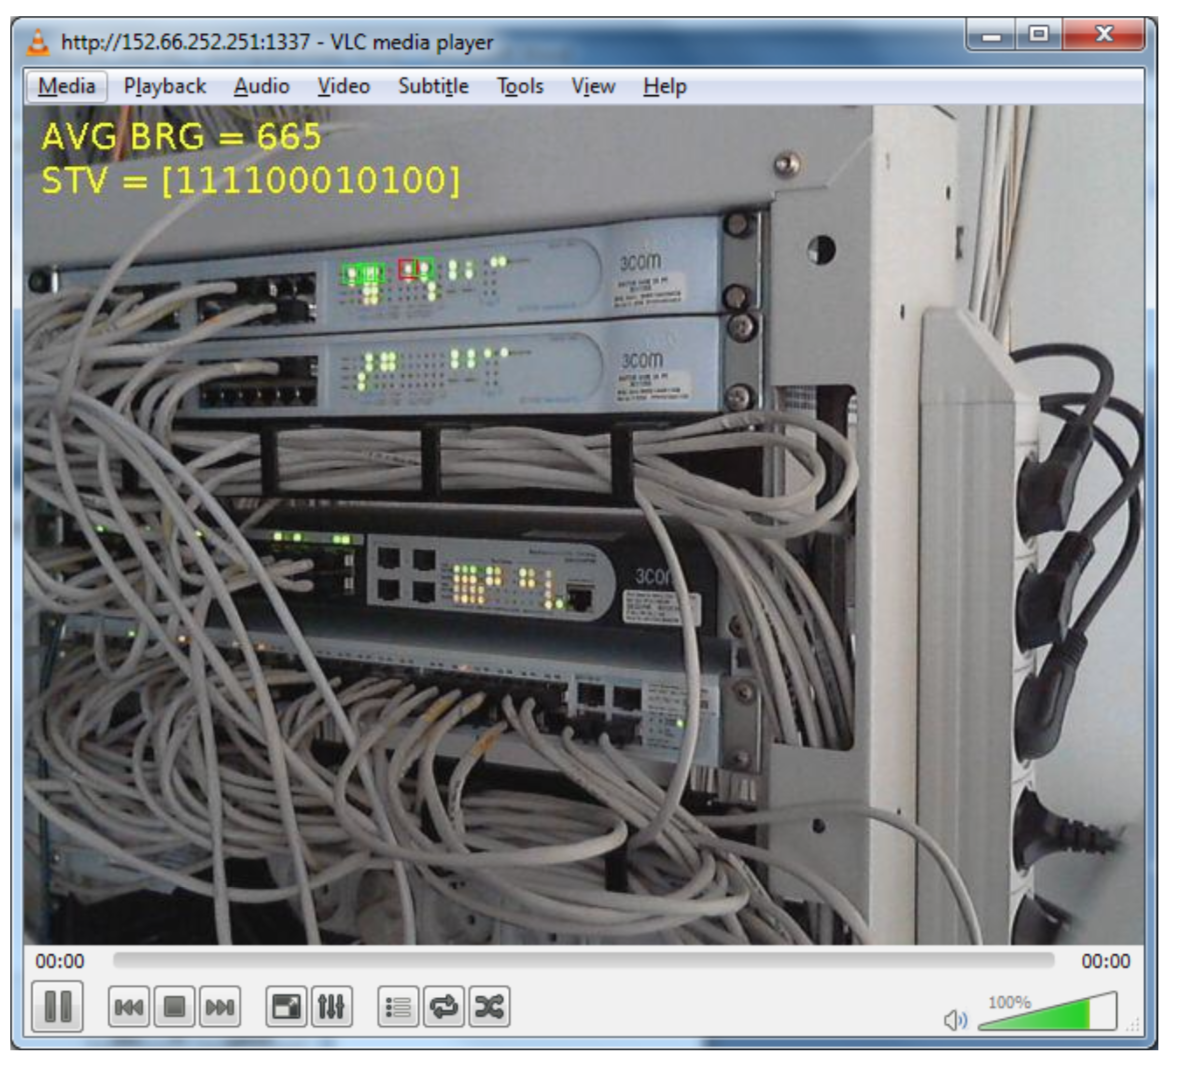
\includegraphics[width=0.9\textwidth]{figures/switchwork.png}
	\caption{Input image and corresponding output vectors\label{fig:switchwork}}
\end{figure}

The measurements are accumulated into a vector which projects each LED's state. Then the state vector is forwarded into the SOS database. The system also recognizes human interaction. If high movement is detected the system does not send the state vector but a marker signal that tells the system that human movement is detected. If there has been no movement for a long time, the system should automatically recover and show the state of the LEDs. The sensor input is stored in a plain text file.

The video capturing is done by a Raspberry PI device. The stream is sent to a Beagleboard computer which is running the the image processing application. It has the text file with the configuration. The text file contain 5 different lines:
\begin{itemize}
	\item[server] the URL of the video stream.
	\item[username] username for password protected streams.
	\item[password] password for the protected stream.
	\item[sos] URL for the POX endpoint of the SOS database.
	\item[point] there can be multiple of this descriptor, which sets the X and Y coordinates of the LEDs
\end{itemize}	
The input image and the output state vector can be seen on Figure \ref{fig:switchwork}.


\section{Building monitoring example application}

The use case is a typical infrastructure monitoring system. It consists of such devices that can be used for intruder detection or measuring usage of certain rooms. It is a demo environment which have been built up in room IE322 and the third floor corridor at the University.
Detailed description of the devices follows.

\subsection*{Microphone}
 The microphone is used for sound analyzing it is used in virtual sensors. It has a streaming output that can be captured or processed further by other sensors. The device's output in SOS is a streaming URL which can be used to listen to the signal. 
 
 It has only one observable property, the stream URL, which is given as a text result by name "observableProperty/stream\_url"
 
 It is placed in IE322 room.
 
 \subsection*{Eco sensor}
 Eco sensors are also physical sensors like the microphone device. They are motion sensors of intruder alert system. For that they have measure several physical properties which ensemble would be used in the output. These observable properties are:
 \begin{itemize}
 \item Temperature: measures temperature near the sensor. It is measured in degrees Celsius. It has the name observableProperty/temperature
 \item Motion: when motion is detected a boolean signal will be sent, which will have true value if motion is detected. The name of this property is observableProperty/motion.
 \item Luminance: Brightness in the room measured by the sensor. It is given in an inner unit as a floating point number. It is named observableProperty/luminance in the database.
 \item Battery voltage: the voltage of the used batteries. It is given in Volts. Using the measurement unexpected power losses can be prevented. Its name in the database is observableProperty/battery\_voltage
 \end{itemize}
 There are 13 eco sensors in the system. 9 of them is in the corridor and 4 is in room IE322.  
 
 \subsection*{Door state sensor}
 These sensors monitor the closeness of windows and doors. They have a boolean property which represent if the door or windows is closed or not. Its only measured property is named observableProperty/door\_state
 It is placed in IE322 room.
 
\subsection*{Speech sensor}

The speech sensor is the only virtual sensor in the system. It listens to the microphone audio stream and tries to decode the sentences that has been said in the monitored room. It gives the decoded text as answer.

\section{Communication between the sensors and the databases}

Each node has some kind of Linux based operating system. The example applications are all Java based, but other platforms will be supported in the future. The sensor measurements are sent using the POX GET requests to the SOS database. The advantage of the GET requests that from a Linux system, new sensor data can be submitted using the curl command even from the command line.  The load data will be sent using the described support services in Section \ref{sec:rdfstore}. The service communicates using JSON objects and POST requests.

This means that each node is communicating with both the databases. From those databases the planner service plans the deployment of new devices and the monitoring system integrates the information of both databases as one information. The monitoring system is described in the next section.

\section{Improvements for the current system}

The system was built as a proof of concept for a cyberphisical system. The system works and proves that such a application can exist, however there are some things that can be improved in the future. 

\subsection{Scalability}

The application should be scalable. The described system is scalable in vertical way, computers with larger processing and storage capacity can serve bigger amount of data. The different services can be deployed to separate servers, however these services can't be distributed. The real solution would be if those services would be horizontally scalable. This means that more computer would provide more capacity to the system. The used PostgreSQL database has a commercial version, which is horizontally scalable, however this can not be used without modifying the SOS servers source code.  

The SOS server is a JAVA enterprise application it is scalable horizontally by deploying the application to multiple computers, however it can't be used with dynamic load balancing, because the session information can not be shared between the instances. The used RDF database has a commercial version which is also scalable.

\subsection{Data integration}

Currently the system communicates to two separate databases. These databases should be merged and provide a common interface towards the sensors which can send measurements and performance information on a common service. Currently the sensors upload measurements using a Java application which is running on the devices, but load reports are uploaded using ssh remote connection. An initiator connects to the device and calls the script which updates the database. This should be integrated on the device, not to depend on external support machines.

In the semantic description two databases has been created. One for the sensor browser, which provides semantic connection between the sensors and one that has the SISRO description of the performance measures. These two databases should be merged into one database and provide a common way for reading and manipulating the data. In the current setup the provided and extended sensor connection description can't be joined with the SISRO database, because the data stored in each database is different. The former is about sensor data the latter is about device load.

\subsection{Authentication}

In the current setup, anyone can post new measurements to the SOS database. The sensors are not authenticated, they can also add data to different sensors dataset or modify its data. The real system should have access rights which would select which user can write which part of the database. The RDF database has basic authentication but all sensors use the same credentials for that. Each sensor can change the data of any sensors.
